% !TEX TS-program = pdflatex
% !TEX encoding = UTF-8 Unicode

% This is a simple template for a LaTeX document using the "article" class.
% See "book", "report", "letter" for other types of document.

\documentclass[11pt]{article} % use larger type; default would be 10pt
    
    \usepackage[utf8]{inputenc} % set input encoding (not needed with XeLaTeX)
    
    %%% Examples of Article customizations
    % These packages are optional, depending whether you want the features they provide.
    % See the LaTeX Companion or other references for full information.
    
    %%% PAGE DIMENSIONS
    \usepackage{geometry} % to change the page dimensions
    \geometry{letterpaper} % or letterpaper (US) or a5paper or....
    % \geometry{margin=2in} % for example, change the margins to 2 inches all round
    % \geometry{landscape} % set up the page for landscape
    %   read geometry.pdf for detailed page layout information
    
    \usepackage{graphicx} % support the \includegraphics command and options
    
    \usepackage[parfill]{parskip} % Activate to begin paragraphs with an empty line rather than an indent
    
    %%% PACKAGES
    \usepackage{booktabs} % for much better looking tables
    \usepackage{array} % for better arrays (eg matrices) in maths
    \usepackage{paralist} % very flexible & customisable lists (eg. enumerate/itemize, etc.)
    \usepackage{verbatim} % adds environment for commenting out blocks of text & for better verbatim
    \usepackage{subfig} % make it possible to include more than one captioned figure/table in a single float
    % These packages are all incorporated in the memoir class to one degree or another...
    \usepackage[sectionbib,square]{natbib}
    
    %%% HEADERS & FOOTERS
    \usepackage{fancyhdr} % This should be set AFTER setting up the page geometry
    \pagestyle{fancy} % options: empty , plain , fancy
    \renewcommand{\headrulewidth}{0pt} % customise the layout...
    \lhead{}\chead{}\rhead{}
    \lfoot{}\cfoot{\thepage}\rfoot{}
    
    %%% SECTION TITLE APPEARANCE
    \usepackage{sectsty}
    \allsectionsfont{\sffamily\mdseries\upshape} % (See the fntguide.pdf for font help)
    % (This matches ConTeXt defaults)
    
    %%% ToC (table of contents) APPEARANCE
    \usepackage[nottoc,notlof,notlot]{tocbibind} % Put the bibliography in the ToC
    \usepackage[titles,subfigure]{tocloft} % Alter the style of the Table of Contents
    \renewcommand{\cftsecfont}{\rmfamily\mdseries\upshape}
    \renewcommand{\cftsecpagefont}{\rmfamily\mdseries\upshape} % No bold!
    
    %%% END Article customization
    
    \begin{document}
    \bibliographystyle{plainnat}

    DynEarthSol3D (DES3D)~\citep{Choi2013,Tan2013,Ta2015,Logan2017} is an explicit dynamic finite element code providing quasi-static solutions to the momentum balance equation via the dynamic relaxation~\citep{Cundall1989} and mass scaling~\citep[e.g.][]{Chung1998}. The explicit formulation makes it easy to implement complex rheologies. The limit on time step size is a drawback associated with an explicit time integration but the mass scaling technique can mitigate it to some degree.
    
    In this project, we are going to use the Mohr-Coulomb elasto-plastic rheology. This rheology is suitable for describing elastic and brittle behaviors of rocks as in \texttt{fdfault} without complications from rate-dependent creep as in viscoelastic or elasto-visco-plastic rheologies. That we can choose to exclude completely time-dependent creep behaviors from consideration not only ensures seamless coupling with \texttt{fdfault} but also must subdue the unwarrented but often-raised doubt about the legitimacy of using \texttt{DES3D} for interseismic time scales of 1-1000 years.
    
    Recent extension of the Mohr-Coulomb rheology in \texttt{DES3D} to the rate-and-state friction [Tong and Lavier, \emph{in prep}] further demonstrates that this code can handle the rheology perfectly relevant to earthquake cycles. In Tong and Lavier's approach, velocity magnitude is evaluated, the state variable is updated based on it and the rate-and-state friction coefficient ($\mu_{RS}$) is computed based on the updated velocity and state variable at each quadrature point of an element. $\mu_{RS}$ is then used in the Mohr-Coulomb failure criterion as well as in the return mapping for stress update. %The explicit formulation of \texttt{DES3D} enables us to implement the rate-and-state friction law without invoking iterative non-linear solution schemes, which are necessary in the usual quasi-static formulation.
    
    In an example showin in Fig.~\ref{fig:RSfriction}, a 10 km-thick layer of elastic crust is sheared to initiate and maintain earthquake cycles. A 2 km-thick pre-existing shear zone is in contact with the crustal layer and composed of the Mohr-Coulomb plastic materials with rate-and-state friction. Due to the shear loading, shear stress elastically accumulates in both layers. When plastic yielding occurs in the shear zone, the coseismic slip and release of elastic stress occurs and the rate-and-state friction governs this stress-releasing process. $\mu_{RS}$ is given as
    \begin{equation}
      \mu_{RS} = \mu_{0} + a\,\ln (V/V_{0}) + b \, \ln (V_{0}\,\theta/L),
    \end{equation}
    where $mu_{0}$ is the reference friction coefficient, $\theta$ is the state variable that evolves in time as $\dot{\theta}=1-V\theta/L$, $V$ is the slip velocity, $V_{0}$ and $L$ are reference velocity and characteristic length scale. In the shown example, we set $\mu_{0}$ = 0.6, $V_{0}$ = 10$^{-6}$ m/s and $L$ = 3 mm. Also, $a$ = 0.015, $b$ = 0.019 for velocity-weakening patch (central 50 km-wide region in the shear zone) while $a$ = 0.0019  and $b$ = 0.0015 for velocity-strengthening patches. As evident in the right panel of Fig.~\ref{fig:RSfriction}, the implemented rate-and-state friction law successfully reproduces the quasi-periodic earthquake cycles.
    
\begin{figure}
 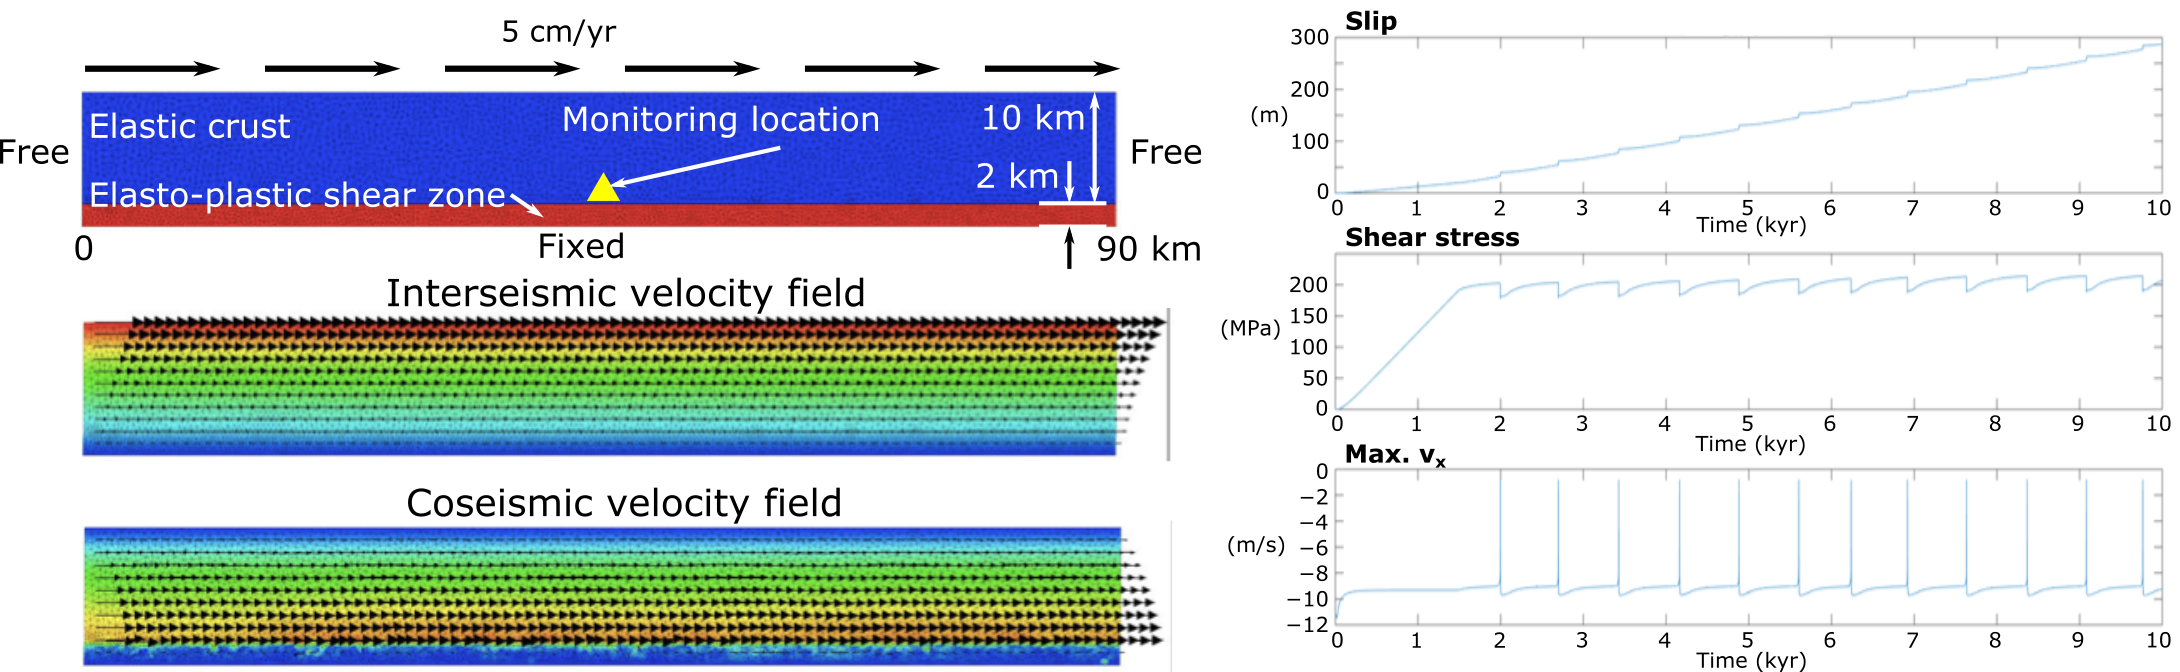
\includegraphics[width=\textwidth]{./RSfriction01.png}
 \caption{(left) Top: Model setup. Middle and bottom: Snapshots of velocity field during interseismic loading and coseismic slip, respectively. (right) Time history of slip, shear stress and maximum velocity magnitude, all of which consistently and clearly exhibit the main characteristics of earthquake cycles.}
 \label{fig:RSfriction}
\end{figure}

    \bibliography{./refs.bib}
    
    \end{document}
    